\section*{Exercice 181 -- Transmission vis-écrou}
\setcounter{exo}{0}

\textit{D'après ressources Pole Chateaubriand -- Joliot-Curie.}

On s’intéresse ici à l’axe Y qui met en mouvement le coulisseau 1,
sur lequel est fixée l’outil, par rapport au bâti 0. Le coulisseau 1 est mis en mouvement par un moteur
électrique qui délivre un couple moteur $C_m(t)$.

\begin{center}
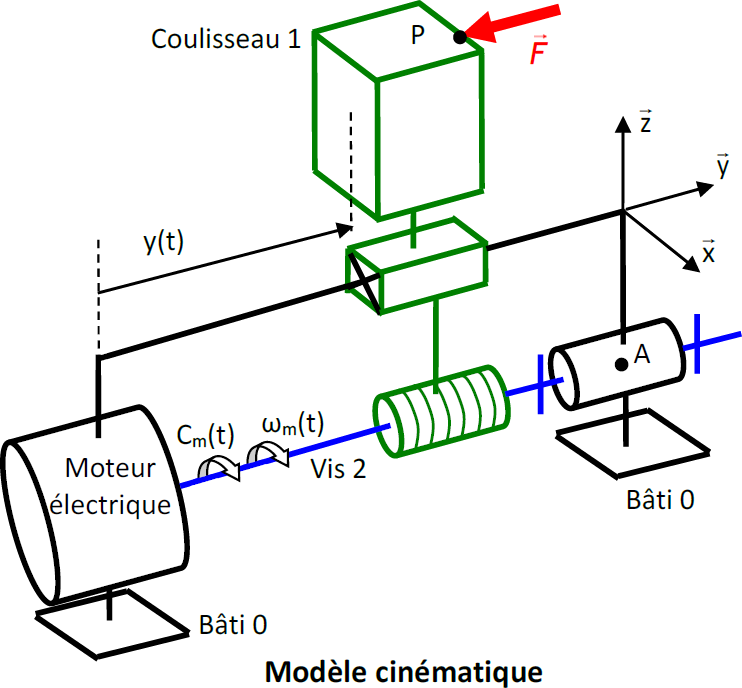
\includegraphics[width=.8\linewidth]{038_01}
\end{center}

On note $p$ le pas de vis. 


\subparagraph{}
\textit{Définir la loi entrée-sortie entre la vitesse de translation du coulisseau et la vitesse de rotation du moteur. }
\ifprof
\begin{corrige}
\end{corrige}
\else
\fi

\subparagraph{}
\textit{Définir la relation liant $C_m$ à $^F$ en faisant l'hypothèse que le rendement est unitaire. }
\ifprof
\begin{corrige}
\end{corrige}
\else
\fi